\section{Mathematical preliminaries} \label{tex:math_prelim}

\cite{Church:1940:A-formulation-of-the-simple-theory-of-types}

In this section the basic definitions and theorems of type-free (\ref{sec:A1}) and simply-typed (\ref{sec:A2}) lambda calculus, based on~\cite{Barendregt:1981:The-Lambda-Calculus:-Its-Syntax-and-Semantics},~\cite{Barendregt:1992:Lambda-Calculi-with-Types} and~\cite{HindleySeldin:2008:Lambda-Calculus-and-Combinators-an-Introduction}, are presented. The last subsection overviews the basic principles of the continuation-passing technique and illustrates them on simple programming examples.

\subsection{Type-free Lambda Calculus} \label{sec:A1}

\begin{definition}[$\lambda$-terms] The set of \textbf{$\lambda$-terms} $\Lambda$ constructed from an enumerable set of variables $V = \{ v, v_1 ,v_2, \dots\}$ is defined inductively as follows:
\begin{center}
$
\begin{array}{rcll}
x \in V & \Longrightarrow & x \in \Lambda &\\
M,N \in \Lambda &  \Longrightarrow & (MN) \in \Lambda & \text{(\textbf{application})}\\ 
 x \in V, M \in \Lambda&  \Longrightarrow  & (\lambda x.M) \in \Lambda & \text{(\textbf{abstraction})}
\end{array} 
$
\end{center}
\end{definition}

In the term $ (\lambda x.M)$, called abstraction, the variable $x$ is the \textbf{argument} of the function and $M$ is the \textbf{body} of the function. %The variable $x$ is \textbf{bound} by $\lambda$ in  $ (\lambda x.M)$.

\begin{example} \label{app:ex1} The following are $\lambda$-terms:
\begin{align*}
& x \\
& (x_1x_2) \\
& (\lambda x. (x_1 x_2)) \\
& (\lambda x_1. (x_1 x_2)) \\
& ((\lambda x. (x_1 x_2)) x_3 ) 
\end{align*}
\end{example}


\begin{remark}[Parenthesis conventions] \label{rem:parcon}
\begin{itemize}
\item application is left-associative
$$MN_1 N_2 \dots N_n \seq (\dots ( (MN_1) N_2 ) \dots N_n)$$
\item  a sequence of $\lambda$-abstractions $\lambda x_1. (\lambda x_2. ( \dots (\lambda x_n. M) )  ) $ is abbreviated as \\ $\lambda x_1 x_2 \dots x_n.M$
$$\lambda x_1 x_2 \dots x_n.M \seq \lambda x_1. (\lambda x_2. ( \dots (\lambda x_n. M) )  )  $$
\item parentheses surrounding the body of an abstraction can be dropped
$$\lambda x_1 x_2 \dots x_n.(M) \seq \lambda x_1 x_2 \dots x_n.M$$
\item outermost parentheses can be dropped 
$$(M) \seq M$$
\end{itemize}
\end{remark}
%application has a higher precedence than abstraction. 
Note that according to the conventions on parentheses, term $\lambda x. MN$ is a more concise way of writing $\lambda x. (MN)$ and is not equivalent to $(\lambda x. M)N$. 

\begin{example} According to Remark~\ref{rem:parcon}, the $\lambda$-terms in Example~\ref{app:ex1} can be written as follows:
\begin{align*}
& x \\
& x_1x_2 \\
& \lambda x. x_1 x_2 \\
& \lambda x_1. x_1 x_2 \\
& (\lambda x. x_1 x_2) x_3 
\end{align*}
\end{example}



\begin{definition}[Free and bound variables] A variable $x$ is \textbf{free} in a $\lambda$-term $M$ if $x$ is not in the scope of $\lambda x$. If $x$ is in the scope of $\lambda x$, it is \textbf{bound}.
\end{definition}

\begin{example} In the term $ (\lambda x. x_1 x_2)$, the variables $x_1$ and $x_2$ are free. In the term $(\lambda x_1. x_1 x_2)$, the variable $x_1$ is bound and the variable $x_2$ is free. In the term $x(\lambda x.x)$, the variable occurs free in the subterm $x$ and bound in the subterm $\lambda x.x$. 
\end{example}

\begin{definition}[Closed $\lambda$-terms] \ 
\begin{enumerate}
\item The set of \textbf{free variables} of $M$, $FV(M)$ is defined inductively as follows:
\begin{align*}
 FV(x)  & = \{ x \} \\
 FV(\lambda x.M)  & = FV(M) - \{ x \} \\
 FV(MN)  & = FV(M) \cup FV(N)
\end{align*}
\item M is \textbf{closed} or a \textbf{combinator}, if $FV(M) = \emptyset$
%\item The result of \textbf{substitution} of $N$ for (the free occurrences of) $x$ in $M$, denoted $x[x:=N]$, is defined as follows ($x \neq y$):
%\begin{center}
%$
%\begin{array}{rcl}
%x[x:=N] & \defeq & N \\
%y[x:=N] &  \defeq & y\\ 
%(PQ)[x:=N]&  \defeq  & (P[x:=N])(Q[x:=N])\\
%(\lambda y.P)[x:=N] & \defeq & \lambda y.(P[x:=N]) \\
%(\lambda x.P)[x:=N] & \defeq & \lambda x.P
%\end{array} 
%$
%\end{center}
\end{enumerate}
\end{definition}

If an equation $M=N$ is provable in the lambda calculus, the provability is denoted by $\lambda \vdash M = N$
or sometimes just by $M=N$.

\begin{definition}[Axioms and rules] For all $M,N, L,Z \in \Lambda$ the following axioms and rules hold:
\begin{prooftree}
\AXC{} \RightLabel{$\beta$-conversion}
\UIC{$(\lambda x.M)N = M[x:=N]$}
\end{prooftree}

\begin{prooftree}
\AXC{}
\UIC{$M = M$}
\end{prooftree}

\begin{prooftree}
\AXC{$M = N$}
\UIC{$N = M$}
\end{prooftree}

\begin{prooftree}
\AXC{$M=N$}
\AXC{$N=L$}
\BIC{$M=L$}
\end{prooftree}

\begin{prooftree}
\AXC{$M=N$}
\UIC{$MZ=NZ$}
\end{prooftree}

\begin{prooftree}
\AXC{$M=N$}
\UIC{$ZM=ZN$}
\end{prooftree}

\begin{prooftree}
\AXC{$M=N$} \RightLabel{rule $\xi$}
\UIC{$\lambda x.M=\lambda x.N$}
\end{prooftree}

\end{definition}

Importantly, substitution $[x:=N]$ in $M$, denoted $M[x:=N]$, is only applicable to the free occurrences of $x$ in $M$. For example,
\begin{align*}
(xy(\lambda x.x))[x:=N] = Ny(\lambda x.x)
\end{align*}

\begin{definition}[Substitution] The result of \textbf{substitution} of $N$ for the free occurences of $x$ in $M$, i.e. $M[x:=N]$, is defined inductively on the structure of $M$ as follows:
\begin{align*}
 x[x:=N] \defeq  \ & N \\
 y[x:=N] \defeq  \ &  y \ \ \text{provided} \ x \nseq y \\
 (\lambda y.M_1)[x:=N] \defeq   \ & \lambda y. (M_1 [x:=N]) \\
 (M_1 M_2)[x:=N] \defeq  \  & (M_1[x:=N])(M_2[x:=N]) \\
 (\lambda x.M_1)[x:=N]  \defeq \ & \lambda x.M_1
\end{align*}

\end{definition}

\begin{lemma}[Substitution lemma] If  $x \nseq y$ and $x \notin FV(L)$, then
\begin{align*}
 M[x:=N][y:=L] \seq M[y:=L][x:=N[y:=L]]
\end{align*}
\end{lemma}
\begin{proof} The proof is by induction on the structure of $M$.
\end{proof}


When performing a substitution $M[x:=N]$, it is necessary to rename those bound variables in $M$ that are free in N. Otherwise, the substitution 
may lead to a false result. For example, without renaming the bound variable $x$ in $\lambda x.xy$, the substitution  $(\lambda x.xy)[y:=x]$ leads to the term $\lambda x.xx$ that acts differently from the desired term, because the free variable $x$ became bound. However, changing $x$ to $z$, for example, before making the substitution, leads to the desired term $\lambda z.zx$. 

\begin{definition}[$\alpha$-conversion] A \textbf{change of bound variable} $x$ in $M$, or an \textbf{$\alpha$-conversion} in $M$, is the replacement of an occurrence of $\lambda x.N$ in $M$ by $\lambda y.(N[x:=y])$, where $y$ does not occur in $N$.
\end{definition}

\begin{definition}[$\alpha$-congruency] $M$ and $N$ are \textbf{$\alpha$-congruent}, denoted $M \congr N$, if one can result from the other by a finite series of changes of bound variables.
\end{definition}

\begin{example}
\begin{align*}
& \lambda x.xy \congr \lambda z.zy \ncongr \lambda x.xx \\
& \lambda xy.yx(\lambda x.x) \congr \lambda xy. yx(\lambda z.z)  \congr \lambda zy. yz(\lambda x.x) \\
& \lambda xy.yx\congr  \lambda zy. yz \congr  \lambda zx. xz \congr \lambda yx. xy 
\end{align*}
\end{example}

It is natural to identify the terms that are $\alpha$-congruent, as they represent the same processes. Moreover, the same processes can be represented by different terms. For example, $\lambda x.Mx$ and $M$ both lead to $MN$ when applied to $N$. Hence, the following rule can be introduced:
\begin{definition}[Extensionality] \textbf{Extensionality} is the following derivation rule, provided $x \notin FV(MN)$:
\begin{prooftree}
\AXC{$Mx = Nx$}
\UIC{$M = N$}
\end{prooftree}
\end{definition}
The extensionality rule allows to prove $\lambda x. Mx = M$. Alternatively,  $\lambda x. Mx = M$ can be considered to be an axiom:
\begin{definition}[$\eta$-conversion] Let $x \notin FV(M)$. Then
\begin{prooftree}
\AXC{} \RightLabel{$\eta$-conversion}
\UIC{$\lambda x. Mx = M$}
\end{prooftree}
\end{definition}

\begin{definition}[$\beta$-normal form]
\begin{enumerate}
\item $M$ is a \textbf{$\beta$-normal form}, if $M$ has no subterm of the form $(\lambda x.L)K$
\item $M$ \textbf{has a $\beta$-normal form}, if there exists an $N$ such that $N$ is a $\beta$-normal form and $N = M$.
\end{enumerate}
\end{definition}

When $M$ is a $\beta$-normal form, it is often said that $M$ is in normal form.

\begin{example} \
\begin{enumerate}
\item $\lambda x.x$ is in normal form.
\item $(\lambda x.x)y$ has a normal form, namely $y$.
\item $(\lambda xy.y)z$ has a normal form, namely $(\lambda y.y)$.
\item $(\lambda xy.x)z$ has a normal form, namely $z$.
\item $(\lambda x.xx)(\lambda y.yy)$ has no normal form.
\end{enumerate}
\end{example}

A notion of reduction on $\Lambda$ is a binary relation on $\Lambda$. The classical notion of reduction $\beta$ is defined as follows:
\begin{definition} $\beta = \{ ( (\lambda x. M)N , M[x:=N] ) | M, N \in \Lambda  \} $
\end{definition}

\begin{definition}[$\beta$-redex, $\beta$-contractum] 
A \textbf{$\beta$-redex} is a term $M$ such that $(M,N) \in \beta$ for some term $N$. In this case $N$ is called \textbf{$\beta$-contractum} of $M$.
\end{definition}

\begin{definition} The notion of reduction $\beta$ induces the following binary relations:
\begin{align*}
\bconv \  & \textbf{one-step } \beta \textbf{-reduction} \\
\bred \  &  \beta \textbf{-reduction} \\
=_{\beta} \  & \beta \textbf{-equality} \text{ (also called } \beta \textbf{-convertibility}\text{)} 
\end{align*}
These relations are inductively defined as follows:
\begin{center}
$
\begin{array}{rcl}
(M,N) \in \beta & \Longrightarrow & M \bconv N \\
M \bconv N &  \Longrightarrow & ZM \bconv ZN \\ 
M \bconv N &  \Longrightarrow & MZ \bconv NZ \\ 
M \bconv N & \Longrightarrow & \lambda x.M \bconv \lambda x.N \\
& & \\
M \bconv N &  \Longrightarrow & M \bred N \\ 
M \bred M & \\ 
M \bred N, N \bred Z & \Longrightarrow & M \bred Z \\
&& \\
M \bred N &  \Longrightarrow & M =_{\beta} N \\ 
M =_{\beta} N & \Longrightarrow & N =_{\beta} M\\ 
M =_{\beta} N, N =_{\beta} Z & \Longrightarrow & M =_{\beta} Z 
\end{array} 
$
\end{center}


%\begin{enumerate}
%\item $(M,N) \in \beta$
%\end{enumerate}

\end{definition}

The notions of $\beta$-redex and $\beta$-equality allow to give an alternative, more formal, definition of $\beta$-normal form:
\begin{definition}[$\beta$-normal form]  
\begin{enumerate}
\item A term $N$ is called a $\beta$-normal form, if $N$ does not contain (as subterm) any $\beta$-redex.
\item A term $N$ is a $\beta$-normal form of $M$, if $N$ is a $\beta$-normal form and $M =_{\beta} N$.
\end{enumerate}
\end{definition}

%\begin{definition}[$\beta$-contractum, $\beta$-redex] Any term of the form 
%\begin{align*} (\lambda x.M)N
%\end{align*}
%is called a \textbf{$\beta$-redex} and the corresponding term
%\begin{align*} M[x:=N]
%\end{align*}
%is called its \textbf{contractum}.
%\end{definition}

%
%\begin{definition}[$\beta$-contracting, $\beta$-reducing]ff
%\end{definition}

The notion of $\beta$-reduction is very important, because it characterizes provability in $\lambda$ and it is Church-Rosser:

\begin{proposition} $M =_{\beta} N$ iff $\lambda \vdash M = N$
\end{proposition}
\begin{proof} See~\cite[p.59]{Barendregt:1981:The-Lambda-Calculus:-Its-Syntax-and-Semantics}.
%\begin{itemize}
%\item Assume $\lambda \vdash M = N$. Use the induction on the length of the proof of $M=N$.
%\item Assume $M =_{\beta} N$. Show by induction on the definition of the relations involved that
%\end{itemize}
\end{proof}


\begin{theorem}[Church-Rosser theorem for $\bred$] If $L \bred M$ and $L \bred N$, then there exists a term $Z$ such that $M \bred Z$ and $N \bred Z$.
\end{theorem}
\begin{proof} See~\cite[p.62]{Barendregt:1981:The-Lambda-Calculus:-Its-Syntax-and-Semantics} or~\cite[p.289]{HindleySeldin:2008:Lambda-Calculus-and-Combinators-an-Introduction}.
\end{proof}
\begin{figure}[h!]
  \centering
    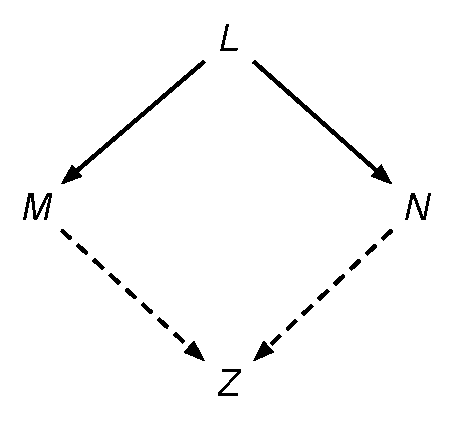
\includegraphics[width=0.3\textwidth]{images/Diamond.pdf}
      \caption{Diamond property.} \label{fig:diamond}
\end{figure}

The Church-Rosser theorem says that for two $\beta$-convertible terms, there is a term to which they both $\beta$-reduce, as illustrated in Figure~\ref{fig:diamond}. The property described in the theorem, that if a term can be reduced to two different terms, then these two terms can be further reduced to one term, is called the \textbf{diamond property} or \textbf{confluence}. The theorem states that $\beta$-reduction is confluent.

\subsection{Simply-typed Lambda Calculus}  \label{sec:A2}

Lambda terms can be assigned expressions, called ``types'', to denote their intended input and output sets. There exists two typing paradigms: 
\`{a} la Curry, sometimes called \textbf{implicit}, and \`{a} la Church, sometimes called \textbf{explicit}. This section first recalls the basics of Curry-style approach and then briefly compares it with the Church-style.

\begin{definition}[Simple types] Given a set $A$ of \textbf{atomic types}, the set of \textbf{types} $T$ is inductively defined as follows:
\begin{center}
$
\begin{array}{rcll}
\alpha \in A & \Longrightarrow & \alpha \in T &\\
\alpha, \beta \in A &  \Longrightarrow & (\alpha \rightarrow \beta) \in T & \text{(\textbf{function types})}
\end{array} 
$
\end{center}
\end{definition}
An atomic type is intended to denote some particular set. A function type $(\alpha \rightarrow \beta)$ is intended to denote some set of functions from $\alpha$ to $\beta$, i.e. the functions that take as the argument a member of the set denoted by $\alpha$ and return as an output a member of the set denoted by $\beta$.


\begin{remark}[Parenthesis convention] A complex functional type $(\alpha_1 \rightarrow (\alpha_2 \rightarrow \dots \rightarrow (\alpha_{n-1} \rightarrow \alpha_n)  \dots ))$ is abbreviated as $\alpha_1 \rightarrow \alpha_2 \rightarrow \dots \rightarrow \alpha_n$ (i.e. parentheses are associated to the right):
\begin{align*}
(\alpha_1 \rightarrow (\alpha_2 \rightarrow \dots \rightarrow (\alpha_{n-1} \rightarrow \alpha_n)  \dots )) & \seq \alpha_1 \rightarrow \alpha_2 \rightarrow \dots \rightarrow \alpha_n
\end{align*}
\end{remark}


\begin{definition}[$\lambda\!\rightarrow$-Curry]
\begin{enumerate}
\item A \textbf{statement} is of the form $M:\sigma$ with $M \in \Lambda$ and $\sigma \in T$. The type $\sigma$ is the \textbf{predicate} and the term $M$ is the \textbf{subject} of the statement.
\item A \textbf{declaration} is a statement with a variable as a subject.
\item A \textbf{basis} is a set of declarations with distinct variables as subjects.
\end{enumerate}
\end{definition}


\begin{definition}[Derivation rules in $\lambda\!\rightarrow$-Curry] A statement $M:\sigma$ is \textbf{derivable} from a basis $\Gamma$, denoted $\Gamma \vdash_{\lambda\rightarrow \text{-Curry}} M: \sigma$ , $\Gamma \vdash_{\lambda\rightarrow} M: \sigma$ or simply $\Gamma \vdash M: \sigma$, if $\Gamma \vdash M: \sigma$ can be produced by the following rules:
 
\begin{prooftree}
\AXC{} \RightLabel{axiom}
\UIC{$\Gamma, x: \alpha \vdash x: \alpha $}
\end{prooftree} 
 
 \begin{prooftree}
\AXC{$\Gamma \vdash M: \alpha \rightarrow \beta$}
\AXC{$\Gamma \vdash N: \alpha$} \RightLabel{app}
\BIC{$\Gamma \vdash MN: \beta$}
\end{prooftree}

\begin{prooftree}
\AXC{$\Gamma, x: \alpha \vdash M:\beta$} \RightLabel{abs}
\UIC{$\Gamma \vdash \lambda x.M: \alpha \rightarrow \beta$}
\end{prooftree}

\end{definition}


%\begin{definition}
%
%\medskip \noindent \textbf{Compatibility rules}:
%
%\begin{prooftree}
%\AXC{} \RightLabel{if $x$ is a variable}
%\UIC{$x \evalto x$}
%\end{prooftree}
%
%\begin{prooftree}
%\AXC{} \RightLabel{if $c$ is a constant}
%\UIC{$c \evalto c$}
%\end{prooftree}
%
%\begin{prooftree}
%\AXC{$M \evalto N$}
%\UIC{$\lambda x. M \evalto \lambda x.N $}
%\end{prooftree}
%
%\begin{prooftree}
%\AXC{$M \evalto \lambda x. K$}
%\AXC{$Q \evalto N$}
%\AXC{$K[x:=N] \evalto O$}
%\TIC{$ MQ \evalto O$}
%\end{prooftree}
%
%\begin{prooftree}
%\AXC{$M \evalto x$}
%\AXC{$Q \evalto N$}
%\BIC{$ MQ \evalto xN$}
%\end{prooftree}
%
%\begin{prooftree}
%\AXC{$M \evalto OK$}
%\AXC{$Q \evalto N$}
%\BIC{$ MQ \evalto OKN$}
%\end{prooftree}
%\end{definition}

\begin{lemma}[Substitution lemma for $\lambda\!\rightarrow$-Curry] \label{lem:substitution-Curry} \
\begin{enumerate}
\item If $\Gamma \vdash M:\sigma$, then $\Gamma[\alpha :=\tau] \vdash M:\sigma[\alpha :=\tau]$.
\item Suppose $\Gamma, x: \sigma \vdash M: \tau$ and $\Gamma \vdash N: \sigma$. Then $\Gamma \vdash M[x:=N]: \tau$.
\end{enumerate}
\end{lemma}
\begin{proof} 
\begin{enumerate}
\item The proof is by induction on the derivation of $M:\sigma$.
\item The proof is by induction on the generation of $\Gamma, x: \sigma \vdash M:\tau$
\end{enumerate}
\end{proof}

The following theorem states that the set of terms having a certain type is closed under reduction:
\begin{theorem}[Subject reduction theorem for $\lambda\!\rightarrow$-Curry] Suppose $M \bred N$. Then 
\begin{center}
$
\begin{array}{rcl}
\Gamma \vdash M: \sigma &\Longrightarrow & \Gamma \vdash N: \sigma
\end{array}
$
\end{center}
\end{theorem}
\begin{proof} See~\cite[p.41]{Barendregt:1992:Lambda-Calculi-with-Types}.
\end{proof}

While in Curry's approach each term is assigned a type after the term has been built, in Church's approach, the type of a term is integrated in the term itself. For example, the term $\lambda x.x$ can be assigned a type according to the Curry and Church styles respectively as follows:
\begin{align*}
& \vdash_{Curry} \lambda x.x: (\sigma \rightarrow \sigma) \\
& \vdash_{Church} \lambda x^\sigma.x: (\sigma \rightarrow \sigma) 
\end{align*}
The term $\lambda x^\sigma.x$ itself is annotated in a Church system by $\sigma$. This means that $\lambda x^\sigma.x$ takes the argument $x$ from the particular set denoted by $\sigma$. In contrast, a Curry system allows each term to have a polymorphic type. For example, the term $\lambda x.x:  (\sigma \rightarrow \sigma)$ denotes the operation of doing nothing regardless how $\sigma$ is instantiated: it can stand, for example, for integers or for booleans. 

\begin{definition}[$T$-annotated $\lambda$-terms] Let $V$ be a set of variables, $T$ be a set of types. The set $\Lambda_T$ of $T$\textbf{-annotated} $\lambda$\textbf{-terms} is defined as follows:
\begin{center}
$
\begin{array}{rcl}
x \in V & \Longrightarrow & x \in \Lambda_T \\
M, N \in  \Lambda_T& \Longrightarrow & MN \in \Lambda_T \\
x \in V, M \in \Lambda_T, \sigma \in T & \Longrightarrow & \lambda x^\sigma.M \in \Lambda_T
\end{array}
$
\end{center}
\end{definition}

The typed lambda calculus  \`{a} la Church is defined similarly to the typed lambda calculus  \`{a} la Curry: an important difference is in the derivation rule corresponding to the abstraction: the abstracted variable is explicitly annotated with a type in the Church-style system.
The explicit annotation of types in Church-style system makes it possible to decide whether a term has a certain type. This is an undecidable question for some Curry systems. On the other hand, a Curry-style system has more power and more flexibility than a Church-style system. For example, the easiest way to answer the question whether an untyped term $M$ has any typed analogues is to re-state the question in Curry's notation. Furthermore, Curry-style systems can be generalized in ways Church-style systems cannot. 

Terms \`{a} la Church can be easily mapped into terms \`{a} la Curry. This is done simply by ``erasing'' all type annotations within the term \`{a} la Church:
\begin{definition} $| \cdot |: \Lambda_T \rightarrow \Lambda$ is defined as follows:
\begin{center}
$
\begin{array}{rcl}
|x|& \defeq & x \\
|MN|& \defeq & |M||N| \\
|\lambda x^{\sigma}.M|& \defeq & \lambda x.|M|
\end{array}
$
\end{center}
\end{definition}
The following proposition states that terms in the Church version project to terms in the Curry version of $\lambda\!\rightarrow$; and that terms in the Curry style can be ``lifted'' to terms in the Church style:
\begin{proposition}  
\ 
\begin{enumerate}
\item Let $M \in \Lambda_T$. Then
\begin{align*}
\Gamma \vdash_{Church} M:\sigma  \ \ \Longrightarrow \ \ & \Gamma \vdash_{Curry} |M|:\sigma
\end{align*}
\item Let $N\in \Lambda$. Then
\begin{align*}
\Gamma \vdash_{Curry} N:\sigma  \ \  \Longrightarrow \ \ & \text{exists } M  \in \Lambda_T  \\
& \text{such that }  \Gamma \vdash_{Church}  M:\sigma \text{ and } |M| \congr N
\end{align*}
\end{enumerate}
\end{proposition}
\begin{proof} Both (1) and (2) are proved by induction on the given derivation.
\end{proof}
See~\cite{Barendregt:1992:Lambda-Calculi-with-Types}  and~\cite{HindleySeldin:2008:Lambda-Calculus-and-Combinators-an-Introduction} for profound introductions to the two typing styles and their detailed comparisons.


\subsection{Continuation} \label{subsec:Continuation}

Montague's program requires the meaning of an expression to be computed compositionally from meanings of its lexical constituents. Dynamics of natural language makes, however, this task non-trivial. A similar kind of problem occurred in the mathematical semantics of programming languages, particularly in formalizing full jumps (``goto'' statements) in a compositional way. To solve this problem, the method of continuations was introduced in~\cite{StracheyWadsworth:1974:Continuations:-A-Mathematical-Semantics-for-Handling-Full-Jumps} to extend the mathematical semantics of programming languages~\cite{ScottStrachey:1971:Toward-a-Mathematical-Semantics-for-Computer-Languages} with a general formalized notion of control of full jumps. According to this method, if the evaluation of a program is in a state $s$, and the following command is $c$, continuation represents the state transition which would be produced up to the end of the program (i.e. the rest of the computation) after performing the state transformation specified by $c$. Every function of a program written in continuation-passing style (CPS) is given as an argument to the continuation of the program with respect to this function. 

\subsubsection{CPS Transformation}

A program can be transformed from direct style to continuation-passing style (CPS).
A possible way of CPS-transforming terms of typed lambda calculus was introduced in~\cite{Plotkin:1975:Call-by-Name-Call-by-Value-and-the-lambda-Calculus}. Plotkin's call-by-value transformation is shown in Definition~\ref{def:CPS-transformation}: 
%Moreover, they showed that for typed $\lambda$-calculus the original terms can be recovered from corresponding CPS-terms.
%~\cite{MeyerWand:1985:Continuation-Semantics-in-Typed-Lambda-Calculi-Summary}
\begin{definition}[CPS-transformation]\label{def:CPS-transformation} Let $o$ be a distinguished type. For each term $t$ of type $\rho$, it is possible to construct its CPS-transformation $\overline{t}$ of type $\overline{\rho}$ in the following way
%
\begin{align*}
\overline{x} & = \lambda \phi^{\rho \rightarrow o}. \phi x^{\rho}  \\
\overline{\lambda x^{\alpha}.N^{\beta}} & = \lambda \phi^{(\alpha \rightarrow \beta)' \rightarrow o}. \phi  (\lambda x^{\alpha'}. \overline{N}^{\overline{\beta \rightarrow o}}) \\
\overline{M^{\alpha \rightarrow \beta}N^\alpha} & = \lambda \phi^{\beta' \rightarrow o}. \overline{M}^{\overline{\alpha \rightarrow \beta} }(\lambda m^{(\alpha \rightarrow \beta)'}. \overline{N}^{\overline{\alpha}}(\lambda n^{\alpha'}.mn \phi)) 
\end{align*}
%
where $\phi$ of type $(\rho' \rightarrow o)$ is a \textbf{continuation} of $t$.

Each type  $\overline{\rho}$ is defined as $(\rho' \rightarrow o) \rightarrow o$, where $\rho'$ is as follows
%
\begin{align*}
\rho' = \left\{
\begin{array}{rl} 
\rho & \text{if } \rho \text{ is basic}\\
{\alpha'} \rightarrow ({\beta}' \rightarrow o) \rightarrow o & \text{if } \rho = \alpha \rightarrow \beta \end{array} \right.
\end{align*}
\end{definition}

For a better understanding of CPS-transformation, it is important to keep the type assignments in mind. That is why terms in Definition~\ref{def:CPS-transformation} are presented together with their types as superscripts. Equations~\eqref{eqs:cps} repeat equations in Definition~\ref{def:CPS-transformation} with types omitted for better readability:
%
\begin{subequations}
\begin{align}
\overline{x} & = \lambda \phi. \phi x \label{eq:var}  \\
\overline{\lambda x.N} & = \lambda \phi. \phi (\lambda x. \overline{N}) \label{eq:abst}\\
\overline{MN} & = \lambda \phi. \overline{M}(\lambda m. \overline{N}(\lambda n.mn \phi)) \label{eq:app}
\end{align} \label{eqs:cps}
\end{subequations}

It is possible to make a CPS-transformation of an application in a way that the argument is evaluated before the function, \eqref{eq:app-nws} shows the corresponding transformation rule:
%
\begin{align}
\overline{MN} & = \lambda \phi. \overline{N}(\lambda n. \overline{M}(\lambda m.mn \phi)) \label{eq:app-nws}
\end{align}

The transformation presented above imposes call-by-value evaluation strategy in the resulting term. According to call-by-value strategy, the argument expression is evaluated before being passed to the function.\footnote{Call-by-value is usually contrasted with call-by-name evaluation strategy. According to call-by-name, the argument of a function is not evaluated before the evaluation of the function. Call-by-value evaluation is chosen here as it is closer to Montague's technique of type raising, as discussed in Section~\ref{sec:ContinuationInNLSemantics}.}

\begin{example} \label{ex:CPS1} Consider a $\lambda$-term $t$ computing  $\sqrt{x^3}$:
% 
\begin{align*}
t = \lambda x. \mathsf{sqrt} (\mathsf{cube} \ x)
\end{align*}
%
where $\mathsf{sqrt}$ is a function computing the square root of its argument and $\mathsf{cube}$ is a function computing the cubic power of its argument. Term $t$ can be CPS-transformed (to call-by-value evaluation style) in the following way:
%
 { \small
 \begin{align}
&\overline{\lambda x. \mathsf{sqrt} (\mathsf{cube} \ x )} \notag \\
 = \ &\lambda \phi. \phi (\lambda x. \overline{\mathsf{sqrt} (\mathsf{cube} \ x})) \tag{by~\eqref{eq:abst}} \\
  = \  & \lambda \phi. \phi (\lambda x. (\lambda \phi'. \overline{\mathsf{sqrt}} (\lambda m.\overline{\mathsf{cube} \ x} (\lambda n. m n \phi') ) ) )\tag{by~\eqref{eq:app}} \\
  = \ & \lambda \phi. \phi (\lambda x. (\lambda \phi'. \overline{\mathsf{sqrt}} (\lambda m. ( \lambda \phi''. \overline{\mathsf{cube}} (\lambda m'. \overline{x} (\lambda n'. m'n' \phi'') ) )   (\lambda n. m n \phi') ) ) )\tag{by~\eqref{eq:app}} \\
  \bred & \lambda \phi. \phi (\lambda x. (\lambda \phi'. \overline{\mathsf{sqrt}} (\lambda m. ( \overline{\mathsf{cube}} (\lambda m'. \overline{x} (\lambda n'. m'n'  (\lambda n. m n \phi') ) ) )   ) ) )\notag \\
  = \ & \lambda \phi. \phi (\lambda x. (\lambda \phi'. \overline{\mathsf{sqrt}} (\lambda m. ( \overline{\mathsf{cube}} (\lambda m'. (\lambda \phi''.\phi'' x) (\lambda n'. m'n'  (\lambda n. m n \phi') ) ) )   ) ) )\tag{by~\eqref{eq:var}} \\
  \bred  &\lambda \phi. \phi (\lambda x. (\lambda \phi'. \overline{\mathsf{sqrt}} (\lambda m. ( \overline{\mathsf{cube}} (\lambda m'. m' x  (\lambda n. m n \phi') ) )  ) ) ) \label{eq:ex1nf}
 \end{align} }
 
The CPS versions of $\mathsf{sqrt}$ and $\mathsf{cube}$ are shown in Equations~\eqref{sqrt} and~\eqref{cube} respectively:
%
\begin{subequations}
\begin{align}
\overline{\mathsf{sqrt}} & = \lambda \phi. \phi ( \lambda x \phi'. \phi ' (\mathsf{sqrt}  x))  \label{sqrt} \\
\overline{\mathsf{cube}} & = \lambda \phi. \phi  (  \lambda x \phi'. \phi ' (\mathsf{cube}  x)) \label{cube}
\end{align} 
\end{subequations}

After substituting $\overline{\mathsf{sqrt}}$ and $\overline{\mathsf{cube}}$ in~\eqref{eq:ex1nf} for~\eqref{sqrt} and~\eqref{cube} and $\beta$-reducing,  the normalized CPS-transformed term shown below is obtained:
%
\begin{align*}  
\overline{t} =\lambda \phi. \phi ( \lambda x \phi'. \phi' (\mathsf{sqrt} (\mathsf{cube} x) ) )
\end{align*} 
\end{example} 

Definition~\ref{def:CPS-transformation} transforms a program in direct style into an equivalent program in CPS. For example, $t$ and $\overline{t}$ return the same result for the same argument $4$, as Equations~\eqref{eq:t4} and~\eqref{eq:CPSt4} in the next example show: 
\begin{example}
\begin{align} 
t(4) & = (\lambda x. \mathsf{sqrt} (\mathsf{cube} \ x))(4) \notag\\
& \bconv \mathsf{sqrt} (\mathsf{cube} \ 4) \notag \\
& =  \mathsf{sqrt} \ 64 \notag \\
& = 8 \label{eq:t4}
\end{align}
%
\begin{align}
\lambda \phi. \overline{t} (\lambda \phi'. \phi' 4 \phi) = \ & \lambda \phi. (\lambda \phi. \phi ( \lambda x \phi'. \phi' (\mathsf{sqrt} (\mathsf{cube} x) ) )) (\lambda \phi'. \phi' 4 \phi) \notag \\
\bconv \ & \lambda \phi.  (\lambda \phi'. \phi' 4 \phi)  ( \lambda x \phi'. \phi' (\mathsf{sqrt} (\mathsf{cube} x) ) ) \notag \\
\bconv \ & \lambda \phi.   ( \lambda x \phi'. \phi' (\mathsf{sqrt} (\mathsf{cube} x) ) ) 4 \phi \notag \\
\bconv \ & \lambda \phi. \phi (\mathsf{sqrt} (\mathsf{cube} 4) )   \notag \\
= \ & \lambda \phi. \phi (\mathsf{sqrt} 64 )   \notag \\
= \ & \lambda \phi. \phi 8   \label{eq:CPSt4}  
\end{align}
\end{example}

\subsubsection{CPS Control} \label{subsubsec:CPSControl}

As demonstrated in the previous section, by simply applying Definition~\ref{def:CPS-transformation} one transforms a program into an equivalent CPS program. However, the advantage of a program written in continuation passing style is that it can be expanded with unusual expressions managing its execution, like non-local transfers of control. For example, one of the possible control expressions of a function can be to  discard all the future of the computation (i.e. its continuation) and return the error as a result of the whole program, in case an error happens within this function. Examples~\ref{ex:divbyzero}--~\ref{ex:CPScontrolfinal} show how it can be done in the case of division by zero.
%
\begin{example} \label{ex:divbyzero}
 Consider a $\lambda$-term $t$ computing  $\sqrt{ \dfrac{x}{y}}$: 
 %
\begin{align}
t = \lambda xy. \mathsf{sqrt} (\mathsf{div} \ x \ y) \label{eq:tstat}
\end{align}
%
During the evaluation of $t$, if the execution of $\mathsf{div}$ leads to an error, the error message is passed to the function $\mathsf{sqrt}$ as the argument. Assuming that $\mathsf{sqrt}$ is defined simply as a square root of its argument, this leads to $\mathsf{sqrt}$ being applied to a value for which it is not defined.  For example, this happens if the second of the arguments given to $t$ is zero:
%
\begin{align}
t(9)(0) & =  (\lambda xy. \mathsf{sqrt} (\mathsf{div} \ x \ y))(9)(0)  \notag \\
& \bconv   (\lambda y. \mathsf{sqrt} (\mathsf{div} \ 9 \ y) ) (0)  \notag \\
& \bconv \mathsf{sqrt} (\mathsf{div} \ 9 \ 0)  \notag \\
& = \mathsf{sqrt} (\mathtt{error} ) \label{sqrterrow}\\
& =  \ ??? \notag
\end{align}

\end{example}

This situation could be handled in the original direct program by adding at the beginning of $\mathsf{sqrt}$ a conditional expression that checks whether the argument is an $\mathtt{error}$ (and returning an  $\mathtt{error}$ in this case) or a number (and calculating the square root of the number in this case). However, this means that, following this style, such a condition would have to be added to all other possible functions of the program. In contrast, the CPS technique allows to provide control to the division function itself in a way that it terminates the whole program when an error occurs during its execution.

It is possible to CPS-transform $t$ according to  Definition~\ref{def:CPS-transformation} and the next example demonstrates this. The transformations of functions $\mathsf{sqrt} $ and $\mathsf{div} $, shown below, are necessary for intermediary steps:
%
\begin{subequations}
\begin{align}
\overline{\mathsf{sqrt}} & = \lambda \phi . \phi ( \lambda x \phi'  . \phi'(  \mathsf{sqrt}  x))  \label{sqrt-3} \\
\overline{\mathsf{div}} & = \lambda \phi . \phi  (  \lambda x \phi' . \phi' ( \lambda y \phi''. \phi '' ( \mathsf{div} \ x \ y))) \label{div-3} 
\end{align} \label{eq:sqrtdiv-3}
\end{subequations}

\begin{example}
 %After substituting $ \overline{\mathsf{sqrt}}$ and $ \overline{\mathsf{div}}$ in~\eqref{eq:exdivbyzero0} with their corresponding terms shown in~\eqref{eq:sqrtdiv-3} and $\beta$-reducing, the normalized CPS-transformed $t$, shown in~\eqref{eq:exdivbyzero}, is obtained:
\begin{small}
\begin{align}
& \overline{\lambda xy. \mathsf{sqrt} (\mathsf{div} \ x \ y)}  \notag \\
= \ & \lambda \phi. \phi ( \lambda x. (\overline{\lambda y. \mathsf{sqrt} (\mathsf{div} \ x \ y)}  ))) \tag{by~\eqref{eq:abst}} \\
= \ & \lambda \phi. \phi ( \lambda x. ( \lambda \phi'. \phi' ( \lambda y. \overline{ \mathsf{sqrt} (\mathsf{div} \ x \ y)}  ))) \tag{by~\eqref{eq:abst}} \\
= \ & \lambda \phi. \phi ( \lambda x. ( \lambda \phi'. \phi' ( \lambda y. ( \lambda \phi''. \overline{ \mathsf{sqrt}} ( \lambda m. \overline{\mathsf{div} \ x \ y}  (\lambda n. mn \phi'')  ))) ))\tag{by~\eqref{eq:app}} \\
 = & \dots  \tag{by~\eqref{eq:app}} \\
 \bred \ &  \lambda \phi. \phi ( \lambda x. ( \lambda \phi'. \phi' ( \lambda y. ( \lambda \phi''. \overline{\mathsf{sqrt}}(\lambda m. \overline{\mathsf{div}}  (\lambda m''. m'' x ( \lambda m'. m' y (\lambda n. mn \phi ''))) ) )) ) ) \label{eq:exdivbyzero0}\\
= & \dots \tag{by~\eqref{sqrt-3} and~\eqref{div-3}} \\
 \bred \ &  \lambda \phi. \phi ( \lambda x \phi'. \phi' ( \lambda y \phi ''. \phi''  (\mathsf{sqrt} ( \mathsf{div} \ x\ y ))))\label{eq:exdivbyzero} 
\end{align}
\end{small}
\end{example}

%\overline{t} & =  \lambda \phi. \phi (\lambda x \phi'. \phi' ( \lambda y \phi''. \phi''(\mathsf{sqrt} (\mathsf{div} \ x \ y) ))) \label{eq:exdivbyzeroCPS}

Since normalized term $\overline{t}$ in~\eqref{eq:exdivbyzero} is obtained from $t$ in~\eqref{eq:tstat} only by applying CPS-transformation definitions, it is equivalent to $t$  and behaves analogously when an error happens inside the division function. To demonstrate it, $\overline{t}$ is ``fed'' in the next example with the same (continuized) arguments 9 and 0 as $t$ in Example~\ref{ex:divbyzero}. The fact that the result is equally undesirable can be seen by comparing Equations~\eqref{sqrterrow} and~\eqref{sqrterrowCPS}:

\begin{example}
\begin{align}
& \lambda \phi'''. \overline{t} (\lambda \phi''''. \phi'''' 9 (\lambda \phi'''''. \phi''''' 0 \phi''')) \notag \\
 = \ & \lambda \phi'''. (\lambda \phi. \phi ( \lambda x \phi'. \phi' ( \lambda y \phi ''. \phi''  (\mathsf{sqrt} ( \mathsf{div} \ x\ y ))))) (\lambda \phi''''. \phi'''' 9 (\lambda \phi'''''. \phi''''' 0 \phi''')) \notag \\
  \bconv  \ & \lambda \phi'''.  (\lambda \phi''''. \phi'''' 9 (\lambda \phi'''''. \phi''''' 0 \phi''')) ( \lambda x \phi'. \phi' ( \lambda y \phi ''. \phi''  (\mathsf{sqrt} ( \mathsf{div} \ x\ y ))))\notag \\  
    \bconv  \ & \lambda \phi'''.  ( \lambda x \phi'. \phi' ( \lambda y \phi ''. \phi''  (\mathsf{sqrt} ( \mathsf{div} \ x\ y )))) 9 (\lambda \phi'''''. \phi''''' 0 \phi''')\notag \\
     \bred  \ & \lambda \phi'''.   (\lambda \phi'''''. \phi''''' 0 \phi''') ( \lambda y \phi ''. \phi''  (\mathsf{sqrt} ( \mathsf{div} \ 9\ y ))) \notag \\ 
 \bconv  \ & \lambda \phi'''.    ( \lambda y \phi ''. \phi''  (\mathsf{sqrt} ( \mathsf{div} \ 9\ y )))  0 \phi'''\notag \\
\bred \ & \lambda \phi'''. \phi''' \mathsf{sqrt} (\mathsf{div} \ 9 \ 0)  \notag \\
 =  \ & \lambda \phi'''. \phi''' (\mathsf{sqrt} (\mathtt{error} )) \label{sqrterrowCPS}\\
 =   \ & ??? \notag
\end{align}
\end{example}

However, an advantage of the CPS-written program~\eqref{eq:exdivbyzero} is that it can be extended with an unusual control due to the fact that it, as well as its functions, have continuations as arguments. Particularly, division can be refined in a way so that when the divisor is zero, it disregards the continuation and immediately returns an error message as a result of the whole program; and otherwise provides the result of the division to its continuation. 
Thus, CPS-transformation of $\mathsf{div}$ can be done not directly by Equation~\eqref{div-3}, but by using its modified version~\eqref{div-4} with a control on whether $y$ is equal to zero or not:
%
\begin{align}
\overline{\mathsf{div}} = \ & \lambda \phi . \phi ( \lambda x \phi'. \phi' ( \lambda y .  \mathsf{if} \ (y =0)  \ \mathsf{then} \ \mathtt{error}  \ \mathsf{else}  \  (\lambda \phi''. \phi'' (\mathsf{div} \ x \ y) )) ) \label{div-4}
\end{align} 

Then, using Equation~\eqref{div-4} in~\eqref{eq:exdivbyzero0}, and following Definition~\ref{def:CPS-transformation} in the rest of the transformation, a new CPS program that has a special treatment for division by zero is obtained, as shown below: 
%
\begin{example}
%\begin{footnotesize}
\begin{align}
& \overline{\lambda xy. \mathsf{sqrt} (\mathsf{div} \ x \ y)}  \notag \\
 = & \dots  \tag{by~\eqref{eq:abst} and~\eqref{eq:app}} \\
 \bred \ &  \lambda \phi. \phi ( \lambda x. ( \lambda \phi'. \phi' ( \lambda y. ( \lambda \phi''. \overline{\mathsf{sqrt}}(\lambda m. \overline{\mathsf{div}}  (\lambda m''. m'' x ( \lambda m'. m' y (\lambda n. mn \phi ''))) ) )) ) )\notag\\
= &  \lambda \phi. \phi ( \lambda x. ( \lambda \phi'. \phi' ( \lambda y. ( \lambda \phi''. ( \lambda \phi . \phi ( \lambda x \phi'  . \phi'(  \mathsf{sqrt}  x)) ) \tag{by~\eqref{sqrt-3}} \\
& \phantom{ \lambda \phi. \phi ( \lambda x. ( \lambda \phi'. \phi' ( \lambda y. ( \lambda \phi''. } (\lambda m. \overline{\mathsf{div}}  (\lambda m''. m'' x ( \lambda m'. m' y (\lambda n. mn \phi ''))) ) )) ) ) \notag \\
\bred \ &   \lambda \phi. \phi ( \lambda x. ( \lambda \phi'. \phi' ( \lambda y. ( \lambda \phi''.  \overline{\mathsf{div}}  (\lambda m''. m'' x ( \lambda m'. m' y (\lambda n.  \phi''(  \mathsf{sqrt}  n)))) ) ))  ) \notag \\
= \ & \lambda \phi. \phi ( \lambda x. ( \lambda \phi'. \phi' ( \lambda y. ( \lambda \phi''.  (\lambda \phi . \phi ( \lambda x' \phi'. \phi' ( \lambda y'.  \mathsf{if} \ (y' =0)  \ \mathsf{then} \ \mathtt{error}  \notag  \\
& \phantom{ \lambda \phi. \phi ( \lambda x. ( \lambda \phi'. \phi' ( \lambda y. ( \lambda \phi''.  (\lambda \phi . \phi ( \lambda x' \phi'. \phi' ( \lambda y'.} 
\mathsf{else}  \  (\lambda \phi'''. \phi''' (\mathsf{div} \ x' \ y') )) ) ) \notag \\
& \phantom{\lambda \phi. \phi ( \lambda x. ( \lambda \phi'. \phi' ( \lambda y. ( \lambda \phi''.}
(\lambda m''. m'' x ( \lambda m'. m' y (\lambda n.  \phi''(  \mathsf{sqrt}  n)))) ) ))  )  \tag{by~\eqref{div-4}} \\
\bconv \ & \lambda \phi. \phi ( \lambda x. ( \lambda \phi'. \phi' ( \lambda y. ( \lambda \phi''. (\lambda m''. m'' x ( \lambda m'. m' y (\lambda n.  \phi''(  \mathsf{sqrt}  n)))) \notag \\
& \phantom{\lambda \phi. \phi ( \lambda x. ( \lambda \phi'. \phi' ( \lambda y. ( \lambda \phi''. } 
( \lambda x' \phi'. \phi' ( \lambda y'.  \mathsf{if} \ (y' =0)  \ \mathsf{then} \ \mathtt{error}  \notag\\
& \phantom{\lambda \phi. \phi ( \lambda x. ( \lambda \phi'. \phi' ( \lambda y. ( \lambda \phi''.( \lambda x' \phi'. \phi' ( \lambda y'.   } 
 \mathsf{else}  \  (\lambda \phi'''. \phi''' (\mathsf{div} \ x' \ y') )) ) ) )))\notag \\
\bconv \ & \lambda \phi. \phi ( \lambda x. ( \lambda \phi'. \phi' ( \lambda y. ( \lambda \phi''. ( \lambda x' \phi'. \phi' ( \lambda y'.  \mathsf{if} \ (y' = 0)  \ \mathsf{then} \ \mathtt{error}  \notag \\
&  \phantom{\lambda \phi. \phi ( \lambda x. ( \lambda \phi'. \phi' ( \lambda y. ( \lambda \phi''. ( \lambda x' \phi'. \phi' ( \lambda y'. }
 \mathsf{else}  \  (\lambda \phi'''. \phi''' (\mathsf{div} \ x' \ y') )) ) \notag \\
& \phantom{\lambda \phi. \phi ( \lambda x. ( \lambda \phi'. \phi' ( \lambda y. ( \lambda \phi''. ( }
 x ( \lambda m'. m' y (\lambda n.  \phi''(  \mathsf{sqrt}  n))) ) )))\notag \\
 \bred \ & \lambda \phi. \phi ( \lambda x. ( \lambda \phi'. \phi' ( \lambda y. ( \lambda \phi''.   ( \lambda m'. m' y (\lambda n.  \phi''(  \mathsf{sqrt}  n))) \notag \\
 & \phantom{\lambda \phi. \phi ( \lambda x. ( \lambda \phi'. \phi' ( \lambda y. ( \lambda \phi''.  }
 ( \lambda y'.  \mathsf{if} \ (y' = 0)  \ \mathsf{then} \ \mathtt{error}  \notag \\
& \phantom{\lambda \phi. \phi ( \lambda x. ( \lambda \phi'. \phi' ( \lambda y. ( \lambda \phi''.   ( \lambda y'.  }  
  \mathsf{else}  \  (\lambda \phi'''. \phi''' (\mathsf{div} \ x \ y') )) ) )))\notag \\
 \bconv \ & \lambda \phi. \phi ( \lambda x. ( \lambda \phi'. \phi' ( \lambda y. ( \lambda \phi''.    ( \lambda y'.  \mathsf{if} \ (y' = 0)  \ \mathsf{then} \ \mathtt{error}  \notag \\
 & \phantom{\lambda \phi. \phi ( \lambda x. ( \lambda \phi'. \phi' ( \lambda y. ( \lambda \phi''.    ( \lambda y'. }
  \mathsf{else}  \  (\lambda \phi'''. \phi''' (\mathsf{div} \ x \ y') )) y (\lambda n.  \phi''(  \mathsf{sqrt}  n)) ) )))\notag \\
  \bconv \ & \lambda \phi. \phi ( \lambda x. ( \lambda \phi'. \phi' ( \lambda y. ( \lambda \phi''.    \mathsf{if} \ (y = 0)  \ \mathsf{then} \ \mathtt{error}  \notag \\
  & \phantom{\lambda \phi. \phi ( \lambda x. ( \lambda \phi'. \phi' ( \lambda y. ( \lambda \phi''.  }
   \mathsf{else}  \  (\lambda \phi'''. \phi''' (\mathsf{div} \ x \ y) )  (\lambda n.  \phi''(  \mathsf{sqrt}  n)) ) ))) \label{eq:exdivbyzeroCPScontrol} 
\end{align}
%\end{footnotesize}
\end{example}

%
Term~\eqref{eq:exdivbyzeroCPScontrol}, abbreviated below as $\overline{t}^{control}$, computes a square root of a result of a division, as programs $t$ and $\overline{t}$ do. However,  $\overline{t}^{control}$ additionally has the control over division by zero. Particularly, when the divisor is equal to zero, $\overline{t}^{control}$, unlike $t$ and $\overline{t}$, terminates with an error. This is demonstrated in Example~\ref{ex:CPScontrolfinal}:
%
\begin{example} \label{ex:CPScontrolfinal}
%\begin{footnotesize}
\begin{align}
& \lambda \phi. \overline{t}^{control} (\lambda \phi'. \phi' 9 (\lambda \phi''. \phi'' 0 \phi)) \notag \\
= \ & \lambda \phi. (\lambda \phi. \phi ( \lambda x. ( \lambda \phi'. \phi' ( \lambda y. ( \lambda \phi''.    \mathsf{if} \ (y = 0)  \ \mathsf{then} \ \mathtt{error}  \notag \\
& \phantom{\lambda \phi. (\lambda \phi. \phi ( \lambda x. ( \lambda \phi'. \phi' ( \lambda y. ( \lambda \phi''.} 
 \mathsf{else}  \  (\lambda \phi'''. \phi''' (\mathsf{div} \ x \ y) )  (\lambda n.  \phi''(  \mathsf{sqrt}  n)) ) )))) \notag \\
 & \phantom{\lambda \phi.} (\lambda \phi'. \phi' 9 (\lambda \phi''. \phi'' 0 \phi)) \notag \\
 \bconv \ & \lambda \phi.  (\lambda \phi'. \phi' 9 (\lambda \phi''. \phi'' 0 \phi)) \notag \\
 & \phantom{\lambda \phi.} ( \lambda x. ( \lambda \phi'. \phi' ( \lambda y. ( \lambda \phi''.    \mathsf{if} \ (y = 0)  \ \mathsf{then} \ \mathtt{error} \notag \\
& \phantom{\lambda \phi.  ( \lambda x. ( \lambda \phi'. \phi' ( \lambda y. ( \lambda \phi''.    } 
 \mathsf{else}  \  (\lambda \phi'''. \phi''' (\mathsf{div} \ x \ y) )  (\lambda n.  \phi''(  \mathsf{sqrt}  n)) ) ))) \notag \\
 \bconv \ & \lambda \phi.   ( \lambda x. ( \lambda \phi'. \phi' ( \lambda y. ( \lambda \phi''.    \mathsf{if} \ (y = 0)  \ \mathsf{then} \ \mathtt{error} \notag \\
 & \phantom{\lambda \phi.   ( \lambda x. ( \lambda \phi'. \phi' ( \lambda y. ( \lambda \phi''.   }
  \mathsf{else}  \  (\lambda \phi'''. \phi''' (\mathsf{div} \ x \ y) )  (\lambda n.  \phi''(  \mathsf{sqrt}  n)) ) ))) 9 (\lambda \phi''. \phi'' 0 \phi) \notag \\
 \bconv \ & \lambda \phi.   ( \lambda \phi'. \phi' ( \lambda y. ( \lambda \phi''.    \mathsf{if} \ (y = 0)  \ \mathsf{then} \ \mathtt{error} \notag \\
 & \phantom{ \lambda \phi.   ( \lambda \phi'. \phi' ( \lambda y. ( \lambda \phi''. }  \mathsf{else}  \  (\lambda \phi'''. \phi''' (\mathsf{div} \ 9 \ y) )  (\lambda n.  \phi''(  \mathsf{sqrt}  n)) ) ))  (\lambda \phi''. \phi'' 0 \phi) \notag \\
  \bconv \ & \lambda \phi.   (\lambda \phi''. \phi'' 0 \phi) ( \lambda y. ( \lambda \phi''.    \mathsf{if} \ (y = 0)  \ \mathsf{then} \ \mathtt{error} \notag \\
  & \phantom{ \lambda \phi.   (\lambda \phi''. \phi'' 0 \phi) ( \lambda y. ( \lambda \phi''.   }  \mathsf{else}  \  (\lambda \phi'''. \phi''' (\mathsf{div} \ 9 \ y) )  (\lambda n.  \phi''(  \mathsf{sqrt}  n)) ) )  \notag \\
  \bconv \ & \lambda \phi.   ( \lambda y. ( \lambda \phi''.    \mathsf{if} \ (y = 0)  \ \mathsf{then} \ \mathtt{error} \ \mathsf{else}  \  (\lambda \phi'''. \phi''' (\mathsf{div} \ 9 \ y) )  (\lambda n.  \phi''(  \mathsf{sqrt}  n)) ) ) 0 \phi \notag \\
    \bred \ & \lambda \phi. \mathsf{if} \ (0 = 0)  \ \mathsf{then} \ \mathtt{error} \ \mathsf{else}  \  (\lambda \phi'''. \phi''' (\mathsf{div} \ 9 \ 0) )  (\lambda n.  \phi(  \mathsf{sqrt}  n))  \notag \\
=  \ & \ \mathtt{error} \notag %\label{errormsg}
\end{align}
%\end{footnotesize}
\end{example}

As already mentioned above, the method of continuation was introduced to give compositional semantics to full jumps in programming languages. Next example illustrates on the example of a simple language that continuation-based interpretation of $\abort$ operation leads to desired evaluation of a program, while a direct interpretation does not:

\begin{example}
Consider a small programming language $L_1$ consisting of variables from set $\vvar$, expressions from set $\expr$, symbols $:=$ and $;$. The language has the following simple grammar, where $S$ stands for a statement:
\begin{align}
S  \defeq \ & \vvar := \expr \ | \notag \\
&  S;S \notag
\end{align}
Let $\state$ be a function mapping variables to natural numbers:
\begin{align}
\state = \ \vvar \rightarrow \mathbb{N} \notag
\end{align}
The statements $S$ in $L_1$ are interpreted with the function $I$ that maps expressions to natural numbers and statements to transformation on states:
\begin{align}
I_{\expr}: \ & \expr \rightarrow \mathbb{N} \notag \\
I_{S}: \ & S \rightarrow (\state \rightarrow \state) \notag 
\end{align}
Then, compositional semantics of this language can be defined as below, where $\xi$ is a state:
\begin{align}
I_{S}(x:=e)\xi = \ & \xi[x := I_{\expr}(e)] \notag \\
I_{S}(S_1;S_2)\xi = \ & I_S(S_2)(I_S(S_1)\xi) \notag 
\end{align}
Consider, for example, the following program written in $L_1$:
\begin{align*}
& x:= 3; \\
& x:= 5
\end{align*}
After the program is evaluated, the final state stores the value $5$ for $x$:
\begin{align}
I_S(x:=3; x:=5)\xi  = \ & I_S(x:=5)(I_S(x:=3)\xi ) \notag \\
= \ & I_S(x:=5) \xi [ x:=3 ]  \notag \\
= \ & \xi [ x:=5] \notag
\end{align}
Assume now that the language $L_1$ is extended with an $\abort$ operation, resulting in new language $L_2$: 
\begin{align}
S  \defeq \ & \vvar := \expr \ | \notag \\
& S;S \ | \notag \\
& \abort \notag
\end{align}
Intuitively, the interpretation of $\abort$ in a state $\xi$ should return the same state:
\begin{align}
I_{S}(\abort)\xi = \xi \notag
\end{align}
It is desirable that the following program, after its termination (due to $\abort$) should store $3$ as the value of $x$:
\begin{align*}
& x:= 3; \notag \\
& \abort; \notag \\
& x:= 5 \notag
\end{align*}
However, evaluating the program according to the rules defined above, 
results in $x$ having the value $5$:
\begin{align}
I_S(x:=3;\abort; x:=5)\xi  = \ & I_S(x:=5)(I_S(x:=3; \abort)\xi ) \notag \\
= \ & I_S(x:=5)(I_S(\abort)(I_S(x:=3) \xi)) \notag \\
= \ & I_S(x:=5)(I_S(\abort) \xi [ x:=3 ] )  \notag \\
= \ & I_S(x:=5) \xi [  x:=3 ] \notag \\
= \ & \xi [ x:=5] \notag
\end{align}
This can be solved by defining compositional semantics using continuations. Then interpretation $I_S$ is of the type $(S \rightarrow \state \rightarrow (\state \rightarrow \state))$ and the semantic rules are as follows:
\begin{align}
I_{S}(x:=e) \xi \phi = \ & \phi(\xi [ x:=I_{\expr}(e)]) \notag \\
I_{S}(S_1;S_2)\xi \phi = \ &  I_S(S_1)\xi(\lambda s.I_{S}(S_2)s \phi) \notag \\
I_{S}(\abort) \xi \phi = \ &\xi \notag
\end{align}
Evaluation of the program according to continuation-based interpetation rules results in $x$ being assigned the desired value $3$:
\begin{align}
I_{S}(x:=3; \abort; x:=5) \xi \phi  = \ & I_{S}(x:=3) \xi ( \lambda s. I_{S}(\abort) s ( \lambda s'. I_{S}(x:=5) \xi \phi )) \notag \\
= \ & I_{S}(x:=3) \xi (\lambda s.s) \notag \\
= \ & \lambda s.s (\xi [x:=3] )  \notag \\
= \ & \xi [x:=3] \notag
\end{align}
When $\abort$ is absent, continuation-based evaluation of the program  correctly assigns the value $5$ to $x$:
\begin{align}
I_{S}(x:=3; x:=5) \xi \phi = \ & \phi(\xi[x:=3][x:=5]) \notag \\
= \ & \phi (\xi [x:=5]) \notag
\end{align}
\end{example}

\subsubsection{Continuation Technique in Natural Language Semantics} \label{subsubsec:ContinuationInNLSemantics}

%Recent research~\cite{deGroote:2001:Type-raising-continuations-and-classical-logic,Barker:2002:Continuations-and-the-Nature-of-Quantification,Barker:2004:Continuations-in-Natural-Language,Shan:2005:Linguistic-Side-Effects,deGroote:2006:Towards-a-Montagovian-Account-of-Dynamics} shows that CPS-transform is a very useful method for formalizing natural language (discourse) semantics.

Continuation-like approaches can already be found in earlier work on formal compositional semantics of natural language. Montague's~\cite{Montague:1973:The-Proper-Treatment-of-Quantification-in-Ordinary-English} technique of type-raising can be seen as using continuation technique for quantifiers to take scope over complete sentences. In this type-raised setting, scope ambiguities (subject wide scope versus object wide scope) correspond to the change of evaluation order of the arguments. This is one of the features that continuation-style allows. Indeed, compare Montague's account of scope ambiguity shown in~\eqref{eq:MS:looooves}, with respectively equations~\eqref{eq:app} and~\eqref{eq:app-nws} of call-by-value continuation-passing-style transformation, repeated below in~\eqref{eq:apppp}, that impose different evaluation order of the arguments:
%
\begin{subequations}
\begin{align}
\I{loves}_{sws} = \ & \lambda OS. S (\lambda x. O (\lambda y. \textbf{love} x y) ) \\
\I{loves}_{ows} = \ & \lambda OS. O (\lambda y. S (\lambda x. \textbf{love} x y) )
\end{align}
\label{eq:MS:looooves}
\end{subequations}
%
\begin{subequations}
\begin{align}
\overline{MN} & = \lambda \phi. \overline{M}(\lambda m. \overline{N}(\lambda n.mn \phi)) \\
\overline{MN} & = \lambda \phi. \overline{N}(\lambda n. \overline{M}(\lambda m.mn \phi)) 
\end{align}
\label{eq:apppp}
\end{subequations}


More recent research confirms that continuation-passing technique is very useful for formalizing natural language (discourse) semantics. For example Barker~\cite{Barker:2002:Continuations-and-the-Nature-of-Quantification} investigates in more details how continuized $\lambda$-terms expressing natural language meanings provide a way of dealing with phenomena related to quantification, such as scope displacement and scope ambiguity, and give a unified account of quantificational and non-quantificational noun phrases. Additionaly, Barker~\cite{Barker:2004:Continuations-in-Natural-Language} shows that CPS can be used to deal with focus, coordination and misplaced quantifiers.\footnote{Other interesting continuation-based analyses of different natural language phenomena include~\cite{Shan:2002:A-continuation-semantics-of-interrogatives-that-accounts-for-Bakers-ambiguity,Shan:2004:Delimited-continuations-in-natural-language,BarkerShan:2008:Donkey-Anaphora-is-In-Scope-Binding}.}

%Although a continuation-passing style allows many apparently non-compositional phenomena to be handled compositionally, it requires type-raising (e.g. an atomic type $\alpha$ becomes $((\alpha \rightarrow o) \rightarrow o) $) and thus result in more complex and less natural $\lambda$-terms and types. However, due to the similarity between type-raising and the double-negation translation (e.g. an atomic proposition $\P1$ becomes $((\P1 \rightarrow \bot) \rightarrow \bot)$), it is possible to obtain more concise and more intuitive lambda terms and types in natural languages semantics by using extended lambda calculi, such as the $\lambda \mu$-calculus~\cite{Parigot:1992:Lambda-My-Calculus:-An-Algorithmic-Interpretation-of-Classical-Natural-Deduction}, originally developed to exploit the double negation translation and provide a Curry-Howard isomorphism for classical logic. This was done in~\cite{deGroote:2001:Type-raising-continuations-and-classical-logic}, where ambiguities in the scope of natural language quantifiers were nicely related to the non-confluence of the $\lambda \mu$-calculus (with $\beta$-, $\mu$- and $\mu'$-reductions), which corresponds to the non-confluence of cut-elimination in classical logic.

Next section proposes an approach that uses continuations in order to implement the influential pragmatic ideas of Stalnaker~\cite{Stalnaker:1978:Assertion} in Montague's settings. This is done by providing two additional arguments to each $\lambda$-term interpreting a natural language proposition. One argument stands for the continuation of the term. Another argument represents a (previously computed) context. Moreover, within the body of the $\lambda$-term, the continuation is applied to the (possibly updated) context (therefore, the continuation is dependent on the context). This is inspired by Stalnaker's idea that each assertion is made in context, is dependent upon the context and updates the context.\footnote{\cite{Heim:1982:The-Semantics-of-Definite-and-Indefinite-Noun-Phrases} and \cite{Kamp:1981:A-Theory-of-Truth-and-Semantic-Representation} also elaborate the work of Stalnaker~\cite{Stalnaker:1978:Assertion}. They do it, however, in a fundamentally different, non-compositional, way. }